% Options for packages loaded elsewhere
\PassOptionsToPackage{unicode}{hyperref}
\PassOptionsToPackage{hyphens}{url}
\PassOptionsToPackage{dvipsnames,svgnames,x11names}{xcolor}
\documentclass[
  11pt,
]{article}
\usepackage{xcolor}
\usepackage[margin=25mm]{geometry}
\usepackage{amsmath,amssymb}
\setcounter{secnumdepth}{-\maxdimen} % remove section numbering
\usepackage{iftex}
\ifPDFTeX
  \usepackage[T1]{fontenc}
  \usepackage[utf8]{inputenc}
  \usepackage{textcomp} % provide euro and other symbols
\else % if luatex or xetex
  \usepackage{unicode-math} % this also loads fontspec
  \defaultfontfeatures{Scale=MatchLowercase}
  \defaultfontfeatures[\rmfamily]{Ligatures=TeX,Scale=1}
\fi
\usepackage{lmodern}
\ifPDFTeX\else
  % xetex/luatex font selection
\fi
% Use upquote if available, for straight quotes in verbatim environments
\IfFileExists{upquote.sty}{\usepackage{upquote}}{}
\IfFileExists{microtype.sty}{% use microtype if available
  \usepackage[]{microtype}
  \UseMicrotypeSet[protrusion]{basicmath} % disable protrusion for tt fonts
}{}
\makeatletter
\@ifundefined{KOMAClassName}{% if non-KOMA class
  \IfFileExists{parskip.sty}{%
    \usepackage{parskip}
  }{% else
    \setlength{\parindent}{0pt}
    \setlength{\parskip}{6pt plus 2pt minus 1pt}}
}{% if KOMA class
  \KOMAoptions{parskip=half}}
\makeatother
\usepackage{graphicx}
\makeatletter
\newsavebox\pandoc@box
\newcommand*\pandocbounded[1]{% scales image to fit in text height/width
  \sbox\pandoc@box{#1}%
  \Gscale@div\@tempa{\textheight}{\dimexpr\ht\pandoc@box+\dp\pandoc@box\relax}%
  \Gscale@div\@tempb{\linewidth}{\wd\pandoc@box}%
  \ifdim\@tempb\p@<\@tempa\p@\let\@tempa\@tempb\fi% select the smaller of both
  \ifdim\@tempa\p@<\p@\scalebox{\@tempa}{\usebox\pandoc@box}%
  \else\usebox{\pandoc@box}%
  \fi%
}
% Set default figure placement to htbp
\def\fps@figure{htbp}
\makeatother
\setlength{\emergencystretch}{3em} % prevent overfull lines
\providecommand{\tightlist}{%
  \setlength{\itemsep}{0pt}\setlength{\parskip}{0pt}}
\usepackage{bookmark}
\IfFileExists{xurl.sty}{\usepackage{xurl}}{} % add URL line breaks if available
\urlstyle{same}
\hypersetup{
  pdftitle={A centered stone and three rotating bands},
  pdfauthor={PolyClank / Kokuno Yumeto},
  colorlinks=true,
  linkcolor={teal},
  filecolor={Maroon},
  citecolor={Blue},
  urlcolor={teal},
  pdfcreator={LaTeX via pandoc}}

\title{A centered stone and three rotating bands}
\author{PolyClank / Kokuno Yumeto}
\date{19 September 2026}

\begin{document}
\maketitle

The most approachable result in this work is a concrete infinite family:
a benzel can be tiled by a single right stone at its center and straight
bones arranged with threefold rotational symmetry. The construction
specifies every bone. Its proof explains why the bones fit, why they do
not overlap, and why their only uncovered cells form the central stone.
This is a specialization of the larger residual-and-repair construction,
with an additional placement and symmetry property. {[}T6, §§2--5; PC,
lines 5--28{]}

\subsection{Why this result is being
presented}\label{why-this-result-is-being-presented}

The project began by pursuing Propp's Problem 7, initially unaware of an
earlier full-solution claim by Akshat Sharma, submitted on 8 September
2026. When that claim came to attention, the recorded decision was to
finish and examine the construction already under development. The
resulting work presents an explicit construction and its validation,
with no claim of first priority. The
\href{https://mathdb.com/p/405267/existence-of-benzel-tilings-with-nonnegative-conway-lagarias}{MathDB
problem record} labels Sharma's submission claimed solved and
independently unverified. {[}S; PV, line 5; T10, lines 25--29{]}

\href{https://arxiv.org/html/2206.06472v4}{Propp's Problem 7} asks
whether a nonnegative Conway--Lagarias invariant suffices to tile an
admissible benzel using right stones and the three orientations of
straight bones, with no left stones. The large construction in the
workbench addresses its residue-zero family. Completing the full
problem's three congruence classes also uses the published
generalized-compression theorem discussed below. The centered theorem
can be understood without that dependency. {[}P; AR, §8; T6, §§2--4{]}

\subsection{The cells and the theorem}\label{the-cells-and-the-theorem}

A cell has integer coordinates \((x,y)\). Equivalently, its barycentric
coordinates are \((x,y,1-x-y)\), whose sum is one. Define

\[
u=y-x,\qquad v=1-x-2y,\qquad w=2x+y-1.
\]

The benzel \(V(a,b)\) consists of the cells for which each of \(u,v,w\)
lies between \(1-a\) and \(b-1\), inclusive. This is the original cell
region, expressed in two coordinates. A right stone is

\[
R(x,y)=\{(x,y),(x+1,y),(x,y+1)\}.
\]

A bone is a set of three consecutive cells in one of the directions
\((1,0),(0,1),(1,-1)\). Write \(H(x,y)\) for the horizontal bone
starting at \((x,y)\). A tiling is a partition of the region into these
actual three-cell sets. {[}T10, lines 33--48; P, §§1--2{]}

\textbf{Centered-one-stone theorem.} Let \(d\ge3\) be an integer, set

\[
t_d=\frac{d(d-1)}2,\qquad h=t_d-1,
\]

and let

\[
W_h(d)=V(d+3h,2d+3h)
=V\!\left(\frac{3d^2-d-6}{2},\frac{3d^2+d-6}{2}\right).
\]

There is an explicitly specified tiling of \(W_h(d)\) with exactly one
right stone, namely \(R(0,0)\), and exactly \(3h(h+d)\) bones. The whole
tiling is invariant under the order-three rotation

\[
\rho(x,y)=(y,1-x-y).
\]

The theorem is the \(h=t_d-1\) family of the written band-packing proof.
The argument below gives a shorter route to its central-stone conclusion
by counting the complement directly. {[}T6, lines 90--160 and 248--267;
PC, lines 21--28{]}

\begin{figure}
\centering
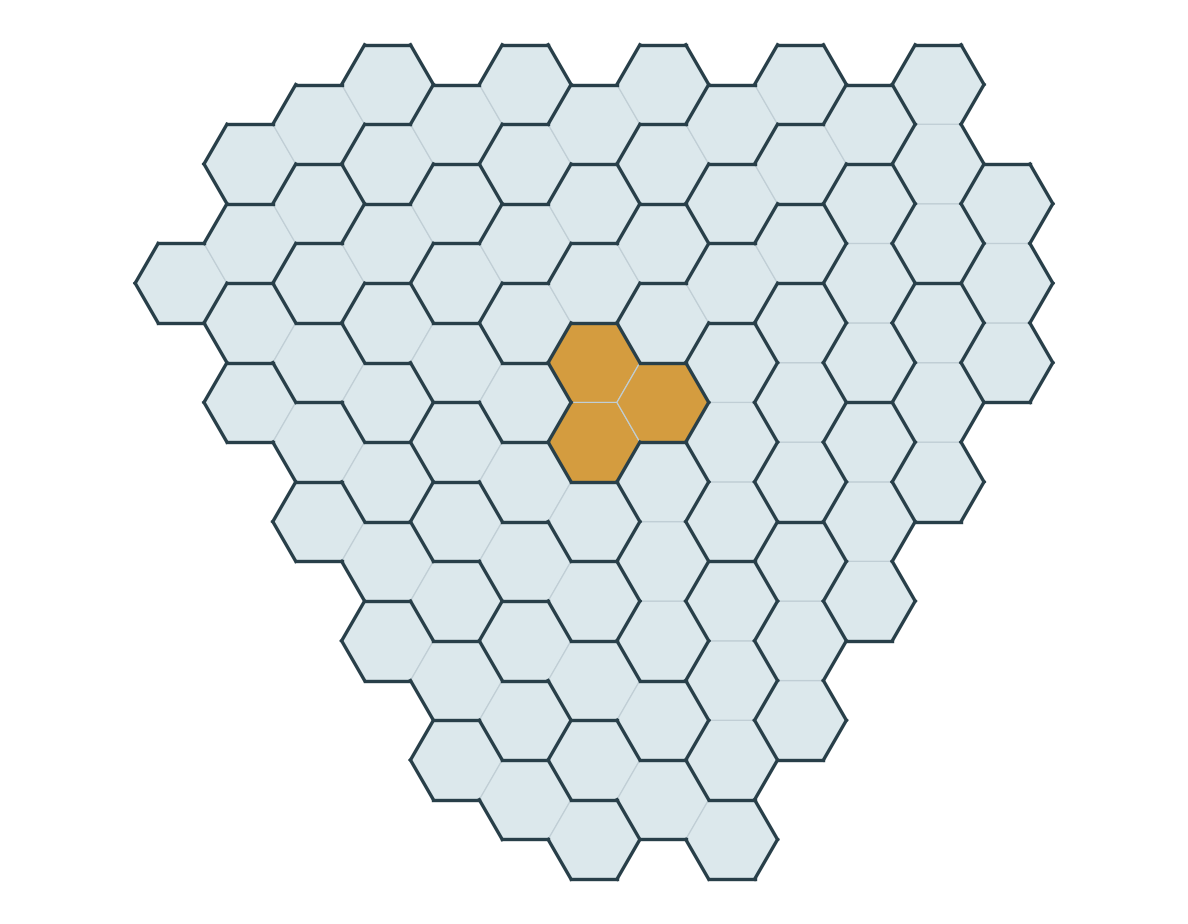
\includegraphics[width=0.7\linewidth,height=\textheight,keepaspectratio,alt={The region V(9,12): one central right stone (gold), 30 bones, and 93 cells. Heavy edges distinguish tiles; faint edges distinguish their cells.}]{centered-example.png}
\caption{The region V(9,12): one central right stone (gold), 30 bones,
and 93 cells. Heavy edges distinguish tiles; faint edges distinguish
their cells.}
\end{figure}

\subsection{An explicit construction}\label{an-explicit-construction}

Let \(r(n)\) be the unique positive integer satisfying

\[
t_{r(n)}<n\le t_{r(n)+1}.
\]

The triangular blocks have lengths \(1,2,3,\ldots\); in particular
\(r(2)=2\). For \(1\le y\le2h+d\), define

\[
(L_y,q_y)=
\begin{cases}
(1-2y-r(y+1),\;y),&y\le h,\\
(y-3h-d+1,\;\min(h,2h+d-y)),&y>h.
\end{cases}
\]

Let \(E\) contain the horizontal bones

\[
H(L_y+3j,y),\qquad 0\le j<q_y.
\]

Thus each row is filled by consecutive, disjoint, length-three
intervals; when \(q_y=0\), the row contributes no bone. Put
\(F(x,y)=(x,1-x-y)\). Take all bones in

\[
\Gamma=F(E)\cup F\rho(E)\cup F\rho^2(E),
\]

and add \(R(0,0)\). Images here mean images of every cell of each placed
tile. Both transformations preserve the permitted tile shapes. The
formulas are the shift-one case of the retained packing, so they are
also a direct recipe for implementing the theorem. {[}T6, lines 40--55
and 90--100; packing.py, \texttt{band} and \texttt{packing}{]}

\subsection{Why this is a tiling}\label{why-this-is-a-tiling}

First check that the bands stay inside the region. It is convenient to
work before reflection, in \(V(2d+3h,d+3h)\), with difference bounds

\[
A=1-2d-3h,\qquad B=d+3h-1.
\]

A prefix-row cell is \((1-2y-r+z,y)\), where \(r=r(y+1)\) and
\(0\le z\le3y-1\). Its three differences are

\[
3y+r-1-z,\qquad r-z,\qquad1-3y-2r+2z.
\]

Since \(y+1\le h+1=t_d\), one has \(1\le r\le d-1\). Taking the two
endpoints of each expression in \(z\) puts all three differences in
\([A,B]\). In a tail row, write \(y=h+\ell\), \(q=\min(h,h+d-\ell)\).
The differences are

\[
3h+d-1-z,\qquad d-3\ell-z,\qquad3\ell-3h-2d+1+2z,
\]

for \(0\le z<3q\). The inequalities \(q\le h\) and \(\ell+q\le h+d\)
give the same bounds. Rotation preserves the bounds, and reflection
exchanges the two benzel parameters. Every displayed bone is therefore
contained in \(W_h(d)\). {[}T6, lines 102--121{]}

Next check that rotating the sectors does not create overlaps. Every
cell in \(E\) has \(y\ge1\) and \(x<y\). A cell common to \(E\) and
\(\rho E\) would have \(1\le x<y\), with both \((x,y)\) and
\((1-x-y,x)\) in \(E\). If both rows are prefix rows, their row bounds
force

\[
r(y+1)\le y-x\le r(x+1).
\]

Monotonicity forces these three integers to equal some \(r\). But
\(x+1\) and \(y+1\) would then belong to the same triangular block of
length \(r\) while differing by \(r\), which is impossible. If the
higher row is a tail and the lower row a prefix, the corresponding
inequalities force \(d\le y-x\le d-1\). If both are tails, they force
simultaneously \(2x+y\le3h+d\) and \(2x+y\ge3h+d+3\). These exhaust the
cases. Rotation gives the same result for the other sector pairs. {[}T6,
lines 123--143{]}

It remains to identify the uncovered cells. One sector contains

\[
\sum_{y=1}^{h}y+
\sum_{\ell=1}^{h+d}\min(h,h+d-\ell)=h(h+d)
\]

bones. The original region has

\[
|W_h(d)|=3(t_d-h)+9h(h+d)=3+9h(h+d)
\]

cells. The general area formula follows by the explicit three-phase
coordinate count in the original proof; each phase has
\(\binom{d+3h}{2}-2\binom h2-\binom{h+1}{2}\) cells. Consequently the
disjoint packing \(\Gamma\) leaves exactly three cells. {[}T6, lines
57--88 and 145--155{]}

Those cells are the central stone. Indeed, \(R(0,0)\) is fixed as a set
by both \(F\) and \(\rho\), and its three cells have differences in
\(\{-1,0,1\}\), so it is inside the benzel. In \(E\), the only possible
central cell is \((0,1)\), since the other central cells have second
coordinate zero. But row one has \(L_1=-3\) and \(q_1=1\), so its cells
have first coordinates \(-3,-2,-1\). Thus \(E\), and hence each
transformed sector, avoids the center. Three missing cells and three
uncovered central cells finish the partition proof. This paragraph is a
direct specialization of the source formulas; it does not require the
general residual-ranking theorem. {[}T6, lines 19--22, 31, 42 and
95--99{]}

Finally, \(\rho F=F\rho^2\), so applying \(\rho\) merely permutes the
three sectors of \(\Gamma\). The central stone is fixed. This proves the
claimed symmetry and completes the theorem. For \(d=3\), \(h=2\), the
region is \(V(9,12)\), and the construction has one central stone and 30
bones, covering 93 cells. {[}PC, lines 21--28; direct substitution in
the theorem{]}

\subsection{What the band slides add}\label{what-the-band-slides-add}

The same final tiling also has a constructive explanation in terms of
moving vacancies. Start from the shift-zero packing. For
\(r=d-2,d-3,\ldots,1\), shift the band

\[
H(1-r^2+3j,t_{r+1})
\quad\longmapsto\quad
H(2-r^2+3j,t_{r+1}),\qquad0\le j<t_{r+1},
\]

and its two rotations. The old interval starts at
\(Q_r=(1-r^2,t_{r+1})\) and ends one cell before
\(P_r=(t_{r+2},t_{r+1})\). The new interval covers \(P_r\) and leaves
\(Q_r\). This is a positive move: shift the rightmost bone into the
current vacancy, then the next bone, continuing to the left. {[}T6,
lines 269--309{]}

The three vacancies move through successive rotational orbits until they
form \(R(0,0)\). Precisely \(3\binom d3\) old bones participate in this
specified sequence, and the resulting bone set equals \(\Gamma\) above.
This gives an explicit transport, without claiming that it is shortest
or that arbitrary tilings of the same benzel are connected by such
moves. {[}T6, lines 290--318; PC, lines 12--17{]}

Algebra records the replacement as
\(\partial(\mathrm{new}-\mathrm{old})=[P_r]-[Q_r]\), where \(\partial\)
adds the cells of each tile. The positive move is essential: a signed
equation by itself permits subtracting tiles that were never present.
The construction proves separately that each removed bone is present and
each inserted bone fits. This is also the role of the positivity checks
in the full residual-and-repair proof. {[}T6, lines 284--309; AR,
§5.3{]}

\subsection{Relationship to the larger result and to
Sharma}\label{relationship-to-the-larger-result-and-to-sharma}

The full written construction has the domain \(d\ge2\),
\(0\le h\le t_d\), and returns \(t_d-h\) right stones and \(3h(h+d)\)
bones. It fills a parameter-dependent residual by explicit repair
families. The centered theorem is its \(\Delta=t_d-h=1\) branch: the
canonical core has \(m=2,q=0\), and the core tiling is the single
central stone. It is a useful standalone subfamily, not another proof of
every parameter case. {[}T10, lines 11--27 and 77--110; PC, lines
5--10{]}

Here \(\Delta\) counts right stones minus left stones. Propp's
Conway--Lagarias invariant measures their total cell-area difference, so
its value on this residue-zero family is \(CL=3\Delta\). The phrase
``invariant one'' in the workbench means \(\Delta=1\), or \(CL=3\) in
Propp's normalization. {[}AR, lines 275--280; P, §1{]}

\href{https://mathdb.com/api/solution-artifacts/35a67ccb-6716-4906-99fe-54ea1784365b/media}{Sharma's
manuscript}, equations (1.15)--(1.17), prescribes the staircase anchor

\[
P(s,d;c,r)=(-d-2s+2+2c+r,\ d+s-2-c-2r,\ s-c+r),
\]

with \(c,r\ge0\), \(c+r\le d-2\), and a deletion order that leaves
\((c,r)=(0,d-2)\) last. On the one-stone ray, \(s=h=t_d-1\), this gives

\[
P_{\mathrm{last}}=(-2h,h-d+2,h+d-2).
\]

Every cell of that prescribed stone has first coordinate \(-2h\) or
\(1-2h\), whereas the central stone has first coordinate zero or one.
Since \(h\ge2\), the stones are disjoint in the same original region.
For \(V(9,12)\), the staircase anchor is \((-4,1,3)\). The manuscript's
original cell bounds and parameter map agree with those here:
\(s=(2a-b)/3=h\), \(d=b-a\). These definitions and the deletion order
were checked directly in the attached manuscript, PDF pages 2, 4, 5 and
6. {[}S, equations (1.1)--(1.2), (1.9), (1.15)--(1.17), §1.5; PC, lines
30--59{]}

A rotationally invariant tiling with just one right stone must put it at
the center: rotation sends its axial anchor \((x,y)\) to \((y,-x-y)\),
and the fixed-anchor equations force \(x=y=0\). Thus the theorem
supplies a definite additional placement and symmetry property relative
to that prescribed staircase output. {[}PC, lines 61--64{]}

For the full Problem 7 assembly, the residue-one class has a direct
all-right-stone partition. The residue-two class uses
\href{https://arxiv.org/html/2403.07663v1}{Defant--Foster--Li--Propp--Young,
Theorem 1.1}. For \(2\le a\le b\le2a\) and \(a+b\equiv2\pmod3\), put
\(n=b+1-a\) and \(j=(2a-b-1)/3\). That theorem counts tilings using
right stones and two allowed bone orientations by a strictly positive
factorial product. Therefore its tilings are permitted here. The full
assembly cites that theorem; the centered result above does not depend
on it. {[}C; AR, §§8.1--8.2{]}

\subsection{Validation status}\label{validation-status}

On 19 September, Lean checked the five constant positive patch
partitions, their non-overlap and all integer translations, the
eight-bone bridge, and the parameter-uniform band identity above. In
particular, \texttt{Benzel.bandSlide\_correct\ :\ Benzel.BandSlideGoal}
now has a compiled proof. Its proof first telescopes an arbitrary row of
horizontal bones, then substitutes the triangular band length. The
coordinate inverses, central-stone comparison and one original
channel-owner formula were also checked. The
\href{https://github.com/KokunoYumeto/benzel-workbench/blob/main/validation/20260919/lean-checked/README.md}{formal
edition} supplies exact statements, source and 39 named transitive axiom
reports. Only Lean's usual \texttt{propext}, \texttt{Classical.choice}
and \texttt{Quot.sound} occur.

A fresh arithmetic replay also checked all 18 exported polynomial
identities, 6,559 affine certificates, and 24 complete
original/reflected tilings, with 13 intentionally invalid inputs
rejected. It used the supplied separate checker implementations and
matched their recorded mathematical results. This replay certifies those
arithmetic and finite checks; it does not replace the unbounded written
argument.
\href{https://github.com/KokunoYumeto/benzel-workbench/blob/main/validation/20260919/fresh-replay/REPLAY.md}{Fresh
replay}

The AI-assisted construction passed the 18 September audit's separately
implemented checks: 18 reconstructed symbolic identities, 274 tile-owner
identities, 6,559 exact rational certificates and a finite sweep of
3,372 tiling certificates. The universal argument rests on the
parameter-preserving identities, source-membership proofs and exhaustive
parameter decomposition. The finite sweep supplies additional
implementation evidence. The present exposition also rederives the
centered packing and gives its shorter complement proof. {[}AR, §§2--6;
proof above{]}

The research and original audit used the same assistant; independent
human review has not been completed. Neither Sharma's complete proof nor
the entire generalized-compression paper was reaudited. The complete
centered theorem and complete constructor have not yet been certified in
Lean. This edition presents a written construction with explicit checks,
and does not establish novelty of the centered property. {[}AR, §§1, 8.2
and 9; PC, lines 61--64; FM, lines 3--21 and 37--40{]}

\subsection{Primary references}\label{primary-references}

\begin{itemize}
\tightlist
\item
  \textbf{{[}P{]}} James Propp, \emph{Trimer covers in the triangular
  grid: twenty mostly open problems}, arXiv:2206.06472v4, §§1--2 and
  Problem 7 in §6. \href{https://arxiv.org/html/2206.06472v4}{Author
  version}.
\item
  \textbf{{[}C{]}} Colin Defant, Leigh Foster, Rupert Li, James Propp
  and Benjamin Young, \emph{Tilings of Benzels via Generalized
  Compression}, Theorem 1.1. SIAM Journal on Discrete Mathematics
  \textbf{39}(1), 146--162 (2025), DOI
  \href{https://doi.org/10.1137/24M1648247}{10.1137/24M1648247}.
  \href{https://arxiv.org/html/2403.07663v1}{Author version}.
\item
  \textbf{{[}S{]}} Akshat Sharma, \emph{A Constructive Proof of Propp's
  Problem 7}, submitted 8 September 2026.
  \href{https://mathdb.com/p/405267/existence-of-benzel-tilings-with-nonnegative-conway-lagarias}{Submission
  and status};
  \href{https://mathdb.com/api/solution-artifacts/35a67ccb-6716-4906-99fe-54ea1784365b/media}{attached
  manuscript}. The placement comparison uses PDF pages 2 and 4--6;
  current submission status was checked on 19 September 2026.
\end{itemize}

\subsection{Workbench references}\label{workbench-references}

T6: stable-packing and transport proof, turn 6, §§1--5. T10: complete
residue-zero construction, turn 10. AR: 18 September reimplementation
audit. PC: parallel-construction comparison. PV: turn-10 provenance
record. FM: original Lean formalization map. The complete paths and
exact line locators are in the
\href{https://github.com/KokunoYumeto/benzel-workbench/blob/main/validation/20260919/CENTERED_ONE_STONE.md\#workbench-source-map}{online
source map}.

\end{document}
